\subsection{Esercizio 27}
Tabulare il numero di valutazioni di funzione richieste per calcolare, mediante la
function del precedente esercizio, l'approssimazione dell'integrale
\[
    I(f) = \int_{0}^{1} sin\left(\frac{1}{0.1+x}\right)\,dx,
\]
utilizzando le formule di Newton-Cotes di grado n = 1, \dots, 7, e 9,
e tolleranze $tol$ = $10^{-2}$, $10^{-3}$, $10^{-4}$, $10^{-5}$, $10^{-6}$.
\newline \textbf{Soluzione:}

Eseguendo lo script \nameref{cod:27} si ottengono i risultati contenuti nella
tabella \ref{tab:27} e nella figura \ref{fig:es27}, che rappresenta il
logaritmo naturale di numero di valutazioni funzionali.
\begin{table}[ht]
    \centering
    \renewcommand\arraystretch{2}
    \begin{tabular}{| l | c c c c c |}
        \hline
        n & $10^{-2}$ & $10^{-3}$ & $10^{-4}$ & $10^{-5}$ & $10^{-6}$ \\
        \hline
        1 & 5         & 65        & 257       & 1025      & 2049      \\
        2 & 33        & 65        & 129       & 257       & 513       \\
        3 & 7         & 13        & 97        & 193       & 385       \\
        4 & 9         & 33        & 129       & 129       & 257       \\
        5 & 11        & 11        & 41        & 161       & 321       \\
        6 & 13        & 13        & 49        & 97        & 193       \\
        7 & 15        & 15        & 29        & 113       & 113       \\
        9 & 19        & 19        & 19        & 37        & 37        \\
        \hline
    \end{tabular}
    \caption{Numero di valutazioni funzionali rispetto a grado e tolleranza usando funzione \lstinline{composita}}
    \label{tab:27}
\end{table}
\FloatBarrier
\begin{figure}[!ht]
    \centering
    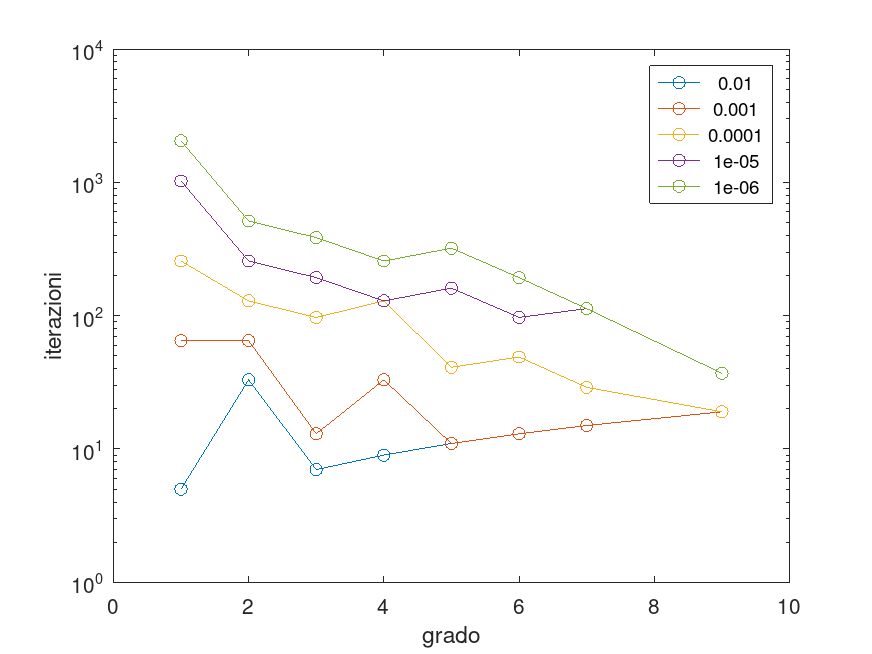
\includegraphics[width=16cm,height=10cm,keepaspectratio]{capitolo5/es27_figure.png}
    \caption{Logaritmo di numero di valutazioni funzionali per funzione \lstinline{composita} rispetto a grado}
    \label{fig:es27}
\end{figure}
\FloatBarrier
